\documentclass[13pt, usenames,dvipsnames]{beamer} %
% \renewcommand{\baselinestretch}{1.3}
\usepackage[T1]{fontenc}
\usepackage{lmodern}
\usepackage{minted}
\usepackage{xcolor}
\usepackage{etoolbox}
\usepackage{tikz}
\usetikzlibrary{fit}
\usepackage{color, colortbl}

\usetikzlibrary{mindmap,trees,shadows}
\tikzset{
  invisible/.style={opacity=0},
  visible on/.style={alt={#1{}{invisible}}},
  alt/.code args={<#1>#2#3}{%
    \alt<#1>{\pgfkeysalso{#2}}{\pgfkeysalso{#3}} % \pgfkeysalso doesn't change the path
  },
}


\definecolor{aliceblue}{rgb}{0.94, 0.97, 1.0}
\definecolor{beige}{rgb}{0.96, 0.96, 0.86}
\definecolor{chartreuse}{rgb}{0.87, 1.0, 0.0}

\usemintedstyle{manni}
\setminted{fontsize=\footnotesize, baselinestretch=1}

\setbeamertemplate{footline}[frame number]
\setbeamercolor{normal text}{fg=black!80,bg=white}
\title{Parallel Computing in Python}
\subtitle{Current State and Recent Advances}
\author{\href{http://kbroman.org}{Pierre Glaser}}


\begin{document}
\begin{frame}[fragile]{}
    \titlepage
\end{frame}

\vspace{3em}

\begin{frame}[t]{}
    \center
    \vspace{3em}
    \tableofcontents[
        subsectionstyle=hide/hide/hide,
        sectionstyle=show
        ]
\end{frame}

\section{Python Interfaces with Parallel Computing}
    \subsection{Python? }
    \begin{frame}[t]{Python? What for?}
        \setbeamercolor{block body}{bg=gray!80}
        \setbeamercolor{frametitle}{bg=gray!80}
        \setbeamercolor{block title}{bg=gray!80}
        \begin{figure}[htpb]
            \vspace*{-0.5cm}
            \hspace*{-1.0cm}
            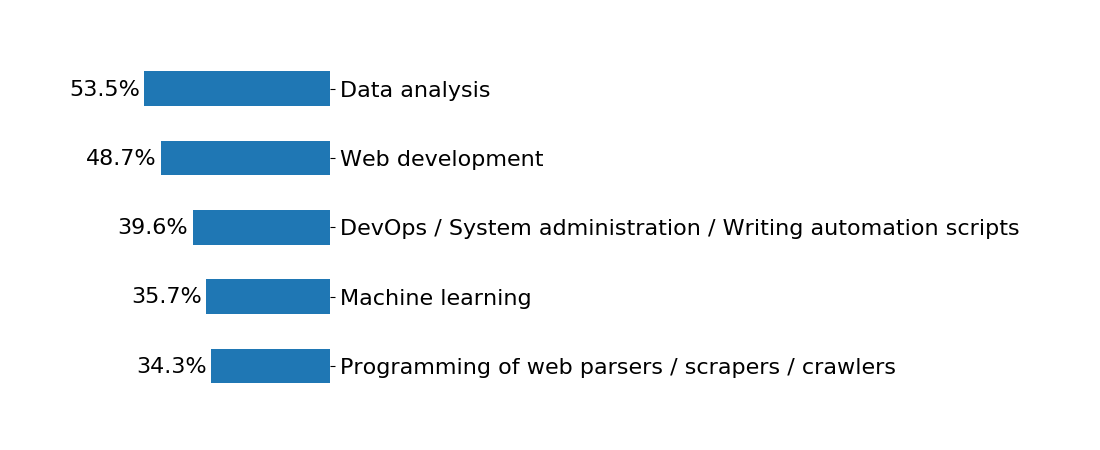
\includegraphics[width=1\linewidth]{media/psf_usage_survey.png}
            \vspace*{-0.5cm}
            \label{fig:media/better_screenshot_python_development_results}
        \end{figure}
        \centering{Python usage among developers
    \footnote{\tiny source: https://www.jetbrains.com/research/python-developers-survey-2018/}
        }
    \end{frame}
    \begin{frame}{A growing scientific computing ecosystem}
        \begin{tikzpicture}
        \node[align=left] (inst) at (1, 0) {%
        
\includegraphics[scale=0.40]{media/scikit-learn-logo.png}};
        \node[align=left] (inst) at (1, -1) {%
        
\includegraphics[scale=0.4]{media/used_by_scikit-learn.png}};
        \node[align=left] (inst) at (8.5, 0) {%
        
\includegraphics[scale=0.30]{media/numpy-logo.png}};
        \node[align=left] (inst) at (8.5, -1.5) {%
        
\includegraphics[scale=0.4]{media/used_by_numpy.png}};
        \node[align=left] (inst) at (4.5, -3) {%
        
\includegraphics[scale=0.40]{media/pandas.png}};
        \node[align=left] (inst) at (4.5, -4.3) {%
        
\includegraphics[scale=0.4]{media/used_by_pandas.png}};
        \end{tikzpicture}
    \end{frame}
    \begin{frame}[t]{Parallel computing? Why?}
        \small
        \vspace{1cm}
        independent, similar computation happens a lot in machine learning.
        \vspace{1cm}
        \begin{itemize}
            \item cross validation
            \item multi-class classification
            \item random forests \tiny{(in general: ensemble models)}
        \end{itemize}
        \vspace{1cm}
        \begin{flushright}
            \small
        Exists for many scikit-learn estimators, but not all.
        \end{flushright}
    \end{frame}
    \begin{frame}[fragile]{User API}
        \small
        Parallelization can be enabled using the \verb|n_jobs| option.
        \begin{beamerboxesrounded}{}
            \begin{minted}[fontfamily=fvm, bgcolor=beige, fontsize=\tiny]{python}
clf = LogisticRegression(solver='saga', n_jobs=4)
X, y = get_data()
clf.fit(X, y)  # runs on 4 cores!
            \end{minted}
        \end{beamerboxesrounded}{}
        \textit{" Let us know if you want to use more CPU resources, because
        parallelizing your models is not hard for you"}
    \end{frame}
    \begin{frame}[fragile]{Multithreading or multiprocessing?}
        Should these separate computations be ran 
        \begin{itemize}
            \item using multiple threads in the main process?
            \item using multiple processes?
        \end{itemize}
    \end{frame}
    \begin{frame}[t]{Cross-validation}
        \footnotesize
        I want to fit the same machine learning model on different subsets of
        the same data.
        \center

        \begin{tikzpicture}
            \tikzset{rounded corners=1}
        \node[align=left, visible on=<1>] (all) at (5, 4) {%
            \begin{tabular}{c c}
                a & b \\
                \hline
                \hline
                1 & 2 \\
                3 & 4 \\
                5 & 6 \\
                7 & 8 \\
        \end{tabular}};
        \node[align=left, visible on=<2>] (all) at (5, 4) {%
            \begin{tabular}{c c}
                a & b \\
                \hline
                \hline
                \rowcolor{beige}
                1 & 2 \\
                3 & 4 \\
                \rowcolor{beige}
                5 & 6 \\
                \rowcolor{beige}
                7 & 8 \\
        \end{tabular}};
        \node[align=left, visible on=<3>] (all) at (5, 4) {%
            \begin{tabular}{c c}
                a & b \\
                \hline
                \hline
                1 & 2 \\
                \rowcolor{aliceblue}
                3 & 4 \\
                \rowcolor{aliceblue}
                5 & 6 \\
                \rowcolor{aliceblue}
                7 & 8 \\
        \end{tabular}};
        \node[align=left, visible on=<4>] (all) at (5, 4) {%
            \begin{tabular}{c c}
                a & b \\
                \hline
                \hline
                \rowcolor{chartreuse}
                1 & 2 \\
                \rowcolor{chartreuse}
                3 & 4 \\
                \rowcolor{chartreuse}
                5 & 6 \\
                7 & 8 \\
        \end{tabular}};
        \node[align=left, visible on=<5->] (all) at (5, 4) {%
            \begin{tabular}{c c}
                a & b \\
                \hline
                \hline
                1 & 2 \\
                3 & 4 \\
                5 & 6 \\
                7 & 8 \\
        \end{tabular}};
        \node[align=left, visible on=<6->] (cv1) at (1.5, 0) {%
                \begin{tabular}{c c}
                    a & b \\
                    \hline
                    \hline
                    \rowcolor{beige}
                    1 & 2 \\
                      &   \\
                    \rowcolor{beige}
                    5 & 6 \\
                    \rowcolor{beige}
                    7 & 8 \\
                \end{tabular}};
        \node[align=left, visible on = <6->] (cv2) at (5, 0) {%
            \begin{tabular}{c c}
                a & b \\
                \hline
                \hline
                  &   \\
                \rowcolor{aliceblue}
                3 & 4 \\
                \rowcolor{aliceblue}
                5 & 6 \\
                \rowcolor{aliceblue}
                7 & 8 \\
            \end{tabular}};
        \node[align=left, visible on=<6->] (cv3) at (8.5, 0) {%
                \begin{tabular}{c c}
                    a & b \\
                    \hline
                    \hline
                    \rowcolor{chartreuse}
                    1 & 2 \\
                    \rowcolor{chartreuse}
                    5 & 6 \\
                    \rowcolor{chartreuse}
                    3 & 4 \\
                      &   \\
                \end{tabular}};
        \node[align=left, visible on = <1->] (worker3) at (8.5, 1.6){%
            \only<-4>{
\includegraphics[scale=0.02]{media/python-logo.png}}
            \only<5-6>{
\includegraphics[scale=0.04]{media/cpu-logo.png}}
            \only<7>{
\includegraphics[scale=0.04]{media/server-logo.png}}};
        \node[align=left, visible on = <1->] (worker2) at (5, 1.6){%
            \only<-4>{
\includegraphics[scale=0.02]{media/python-logo.png}}
            \only<5-6>{
\includegraphics[scale=0.04]{media/cpu-logo.png}}
            \only<7>{
\includegraphics[scale=0.04]{media/server-logo.png}}};
        \node[align=left, visible on = <1->] (worker1) at (1.5, 1.6){%
            \only<-4>{
\includegraphics[scale=0.02]{media/python-logo.png}}
            \only<5-6>{
\includegraphics[scale=0.04]{media/cpu-logo.png}}
            \only<7>{
\includegraphics[scale=0.04]{media/server-logo.png}}};
        % {\draw[->, visible on=<5->] (all.south)--(cv1.north east);}
        % {\draw[->, visible on=<6->] (all.south)--(cv2.north);}
        % {\draw[->, visible on=<7->] (all.south)--(cv3.north west);}
        {\draw[->, visible on=<2>] (worker1.east)--(all.south);}
        {\draw[->, visible on=<3>] (worker2.north)--(all.south);}
        {\draw[->, visible on=<4>] (worker3.west)--(all.south);}
        % {\draw[->, visible on=<3->] (all.south)--(cv2.north);}
        % {\draw[->, visible on=<4->] (all.south)--(cv3.north west);}
        \node[visible on =<1-4>, draw,inner sep=5mm,fit=(all) (worker2) (worker3) (worker1)] {};
        \node[visible on =<5->, draw,inner sep=1mm,fit=(all) (all) (all) (all)] {};
        \node[visible on =<6->, draw,inner sep=1mm,fit=(worker1) (cv1) (cv1) (cv1)] {};
        \node[visible on =<6->, draw,inner sep=1mm,fit=(worker2) (cv2) (cv2) (cv2)] {};
        \node[visible on =<6->, draw,inner sep=1mm,fit=(worker3) (cv3) (cv3) (cv3)] {};


        \node[visible on = <5->, align=left] (legend) at (8, 5){};
        \node[visible on = <5->, align=left] (title) at (9.5, 5){\tiny : single python interpreter};
        \node[draw,inner sep=1mm,fit=(legend) (legend) (legend) (legend)] {};

        \node[visible on = <1-4>, align=left] (backend) at (2, 5){\footnotesize using many threads};
        \node[visible on = <5-6>, align=left] (backend) at (2, 5){\footnotesize using many processes};
        \node[visible on = <7>, align=left] (backend) at (2, 5){\footnotesize using many machines};
        \end{tikzpicture}
    \end{frame}
    \begin{frame}[t]{}
        \center
        \vspace{3em}
        \tableofcontents[
            % currentsubsection,
            % hideothersubsections,
            subsectionstyle=show/hide/hide,
            sectionstyle=show/hide
            ]
    \end{frame}
    \begin{frame}[t]{Different challenges}
        \vspace{2cm}
        \begin{columns}
            \begin{column}{0.5\textwidth}
                \small
                multiprocessing
                \begin{itemize}
                    \item speed (of data communication)
                    \item memory footprint (of duplicated data)
                    \item ease of use, safety (deadlocks)
                \end{itemize}
            \end{column}
            \begin{column}{0.5\textwidth}
                \small
                threading\\
                \vspace{1cm}
                Python usually prevents multiple python threads from running
                simulateously.
            \end{column}
        \end{columns}
    \end{frame}
    \begin{frame}[t]{}
        \vspace{5em}
        \center disclaimer: this talk is mostly cpython specific.
    \end{frame}

    \begin{frame}[t]{In practice}
        \begin{figure}[htpb]
            \centering
            \only<1>{\includegraphics[width=\linewidth]{media/plots/benchmark_plots/seq_vs_parallel_bounds_only.png}}%
            \only<2>{\includegraphics[width=\linewidth]{media/plots/benchmark_plots/seq_vs_parallel_bounds_and_scatter.png}}%
            \only<3>{\includegraphics[width=\linewidth]{media/plots/benchmark_plots/seq_vs_parallel_bounds_and_scatter_and_patches.png}}
            % \caption{Seq vs parallel bounds only}
            \label{seq_vs_parallel_bounds_only}
        \end{figure}
    \end{frame}

    % \subsection{At which level?}
    %     \begin{frame}[t]{The Python Interpreter}

    %     \end{frame}
    %     \begin{frame}[t]{Parallelism at the Python level}

    %     \end{frame}
    %     \begin{frame}[t]{Parallelism at the C level}
    %     \end{frame}
    % \subsection{Using which code?}
    %     \begin{frame}[t]{The python virtual machine}

    %     \end{frame}
    %     \begin{frame}[t]{Arbirtray code execution}

    %     \end{frame}
    %     \begin{frame}[t]{Consequences for paralle computing}

    %     \end{frame}
    % \subsection{In practice?}
    %     \begin{frame}[t]{several matrix-matrix multiplication}
    %         \begin{itemize}
    %             \item using python threads
    %             \item using python processes
    %             \item using BLAS parallelism
    %         \end{itemize}
    %     \end{frame}



\section{Built-in and Third Party ressources}
    \subsection{In the Standard Library}
        \begin{frame}[t]{multiprocessing}

        \end{frame}
        \begin{frame}[t]{concurrent futures}

        \end{frame}
    \subsection{Third party extensions}
        \begin{frame}[t]{loky}

        \end{frame}
        \begin{frame}[t]{joblib}

        \end{frame}
    \subsection{From one to another}
        \begin{frame}[t]{going upstream}

        \end{frame}

\section{Recent Advances}
\subsection{Why we need better IPC}
\subsection{Better extensibility of the pickle module}
\subsection{PEP 574}
    \begin{frame}[t]{principle}
    \end{frame}

    \begin{frame}[t]{better memory footrpint}
    \end{frame}

    \begin{frame}[t]{better speed}
    \end{frame}
\subsection{built-in shared memory in the standard library}



\begin{frame}[fragile]{}
    \setbeamercolor{block body}{bg=beige}
    \begin{beamerboxesrounded}{}
        \inputminted[fontfamily=fvm, bgcolor=beige]{python}{scripts/test_script.py}
    \end{beamerboxesrounded}
\end{frame}
\end{document}
